\documentclass[runningheads]{llncs}
\usepackage[utf8]{inputenc}
\usepackage{graphicx}
\usepackage{float}
\usepackage{subcaption}
\usepackage{hyperref}
\captionsetup{compatibility=false}

\pdfinfo{
/Title (2018 Formatting Instructions for Authors Using LaTeX)
/Author (Felix Linker)}

\begin{document}
    \title{Industrial Benchmark for \\Fuzzy Particle Swarm Reinforcement Learning}

    \author{Felix Linker}

    \authorrunning{F. Linker}

    \institute{Leipzig University, 04109 Leipzig, Germany}

    \maketitle
    \begin{abstract}
        This paper summarizes the results of applying the industrial benchmark to the approach of fuzzy particle swarm reinforcement learning (FPSRL) as proposed in \cite{Hein2017}.
    \end{abstract}


    \section{Introduction}

    The FPSRL approach tries to solve the problem of finding control policies to real world problems by machine learning.
    We recommend to read the paper for a detailed explanation but in short, the approach takes the following steps:

    \begin{enumerate}
        \item Gather real world data of the e.g. industrial plant you want to generate a control strategy for by just measuring its performance
        \item Generalize this data to a world model turning the data gathered into a reward function
        \item Use particle swarm optimization to find an optimal policy regarding this generalized world model
        \item If the performance in the generalized model of the policy is sufficient, evaluate the policy in the real world
    \end{enumerate}

    We implemented this approach to benchmark it with the Industrial Benchmark\footnote{\url{https://github.com/siemens/industrialbenchmark}} \cite{Hein2017a}.
    The Industrial Benchmark tries to give a benchmarking environment for real world industrial plants.
    It generates output from a high-dimensional and hidden state-space, only a part of which is observable.
    In this repository we used the Industrial Benchmark to generate data to create a world model, thus simulating real world runs of some industrial plant and evaluate generated policies.

    By doing so, we implemented an benchmarking approach that was proposed in \cite{Hein2018} for an algorithm that implements the same approach as FPSRL but uses genetic programming instead of particle swarm optimization to search for a policy.

    \section{Results}

    \subsection{World Model}

    The industrial benchmark has an observable state of 4 dimensions.
    When you apply a 3-dimensional action vector to it, the internal state changes which in almost all cases also results in a different observable state.
    The benchmark also yields two performance indicators: a value for fuel costs and consumption costs, latter of which indicate a metric comparable to wear.

    We used two neural networks to predict each of these output variables in time series predicion by implementing an approach as described in \cite{Duell2012} and \cite{Hein2017b} which in turn are referenced by \cite{Hein2017a}.
    The networks were trained on a dataset of which 30\% have been used for validation.
    The world models mean absolute errors on a time series were as follows:

    \begin{center}
        \begin{tabular}{c c}
            Fuel model & Consumption model \\ \hline
            $ 6.11449 $ & $ 18.87096 $
        \end{tabular}
    \end{center}

    It is to no surprise that the prediction of the consumption costs is worse than the prediction of fuel costs as in \cite{Hein2017b} the authors noted that it took more past observations of the state space to accurately predict the consumption costs as opposed to predicting fuel costs.

    In figure \ref{fig:fuel-prediction-examples} and \ref{fig:consumption-prediction-examples} we appended some figures that illustrate time series predictions.

    \subsection{Policy}

    A policy then was generated by a particle swarm in ring topology.
    In total, our policy had $ 84 $ weights thus leading to a $ 84 $-dimensional space that was traversed by 25 particles over 250 iterations.
    We found that quite quickly, after about 100 iterations, the best solution would have been found and further iterations wouldn't increase the solution's quality.
    We also found that using more particles didn't improve results.

    We used the almost the same methods as proposed in \cite{Hein2018} to evaluate a policy with the only difference being that our performance was a cost and positive value leading to a minimization problem whereas the original performance was measured in negative rewards leading to a maximization problem.
    We evaluated our generated policy against the mean performance of 20 randomly generated policies with the following results:

    \begin{center}
        \begin{tabular}{c c}
            Policy performance & Mean random policy performance \\ \hline
            $ 1866.5951 $ & $ 6215.69734 $
        \end{tabular}
    \end{center}

    Although the authors in \cite{Hein2018} didn't give all parameters to their reward function, they considered a successful policy to have costs lower or equal to $ 165 $ which is far from close to our results.
    An explanation for this would be that the approach of geneticly programming algorithms as a policy could utilize the whole past observations history of states whereas the FPSRL policy only inspects the last state.
    Inspecting the whole history of observed states in this case might lead to a policy-state-space one magnitude bigger than the current one - depending on the implementation.

    The authors in \cite{Hein2018} were able to tackle this problem by limiting the complexity of the algorithms.
    The algorithms could choose a number of parameters from past oberservations to calculate their output but as the complexity of the algorithms was limited, they couldn't use \textit{all}.
    This allowed them to use long histories of past oberservations whilst not introducing huge vectors to weigh all those inputs.

    In future, it might be worthwhile to investigate how such an optimization could be applied to the FPSRL approach.

    \section{Implementation}

    All code was written in python and can be found alongside example results and configuration files here: \url{https://github.com/felixlinker/IB_FPSRL}.
    We used keras\footnote{\url{https://keras.io/}} with the tensorflow\footnote{\url{https://www.tensorflow.org/}} backend to implement the world model generation.
    We used pyswarms \cite{Miranda2018} to implement the particle swarm optimization.

    \newcommand{\figwidth}{0.45\textwidth}

    \begin{figure}[hp]
        \centering
        \begin{subfigure}{\figwidth}
            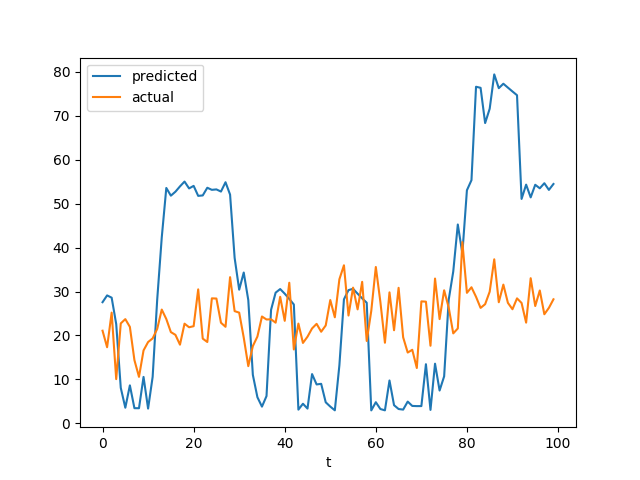
\includegraphics[width=\textwidth]{results/evaluation/f_model_graph_p10.png}
        \end{subfigure}
        \begin{subfigure}{\figwidth}
            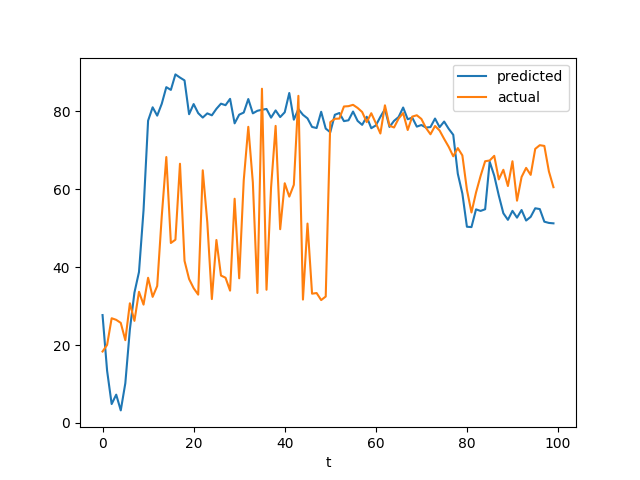
\includegraphics[width=\textwidth]{results/evaluation/f_model_graph_p20.png}
        \end{subfigure}
        \begin{subfigure}{\figwidth}
            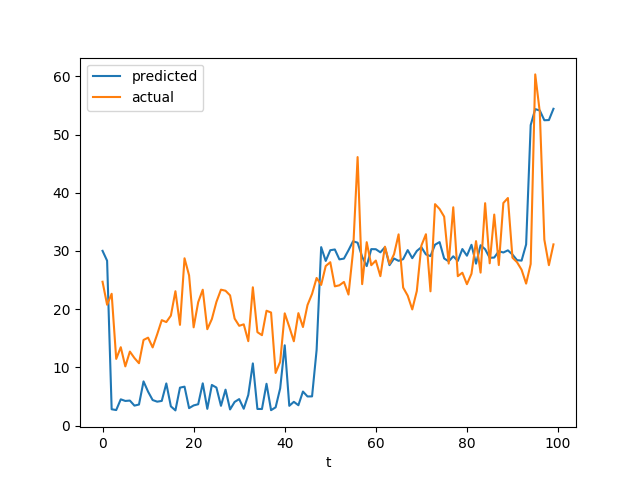
\includegraphics[width=\textwidth]{results/evaluation/f_model_graph_p30.png}
        \end{subfigure}
        \begin{subfigure}{\figwidth}
            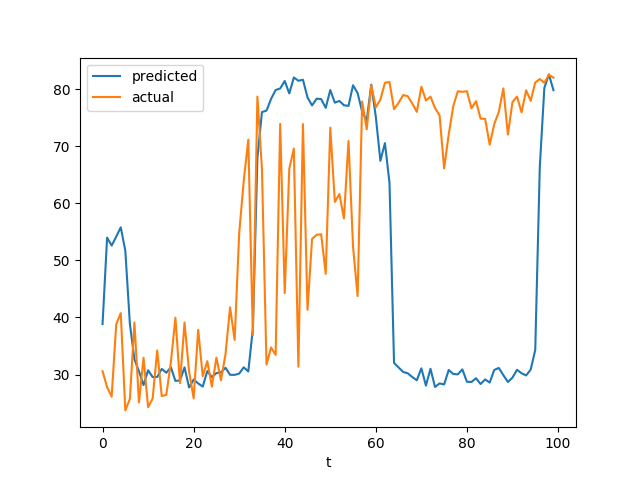
\includegraphics[width=\textwidth]{results/evaluation/f_model_graph_p40.png}
        \end{subfigure}
        \begin{subfigure}{\figwidth}
                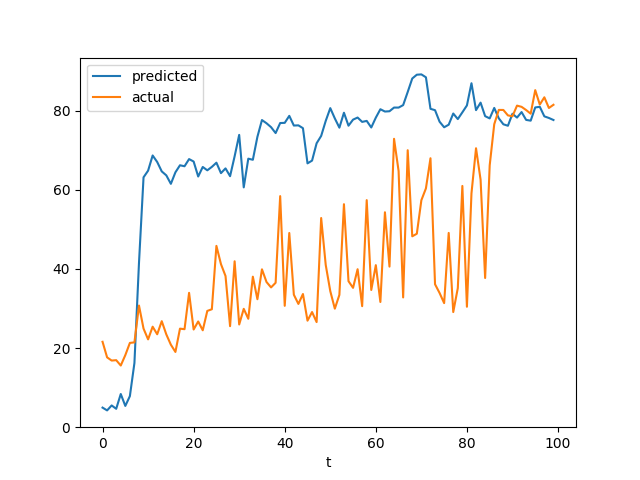
\includegraphics[width=\textwidth]{results/evaluation/f_model_graph_p50.png}
        \end{subfigure}
        \begin{subfigure}{\figwidth}
                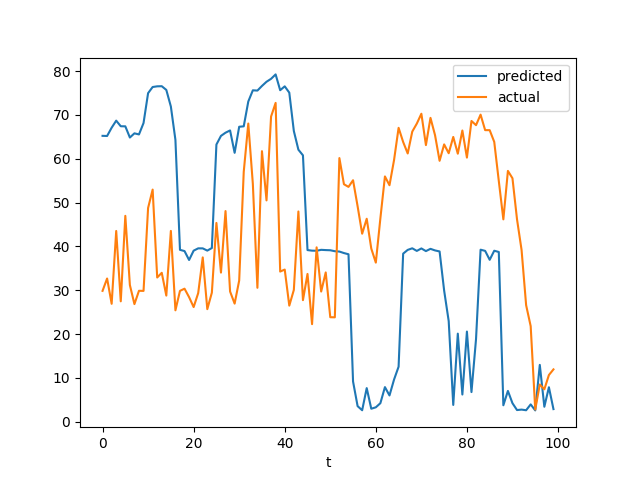
\includegraphics[width=\textwidth]{results/evaluation/f_model_graph_p60.png}
        \end{subfigure}
        \begin{subfigure}{\figwidth}
                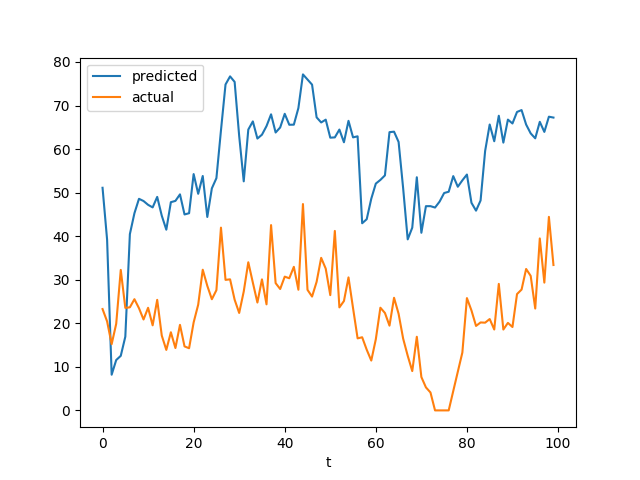
\includegraphics[width=\textwidth]{results/evaluation/f_model_graph_p70.png}
        \end{subfigure}
        \begin{subfigure}{\figwidth}
                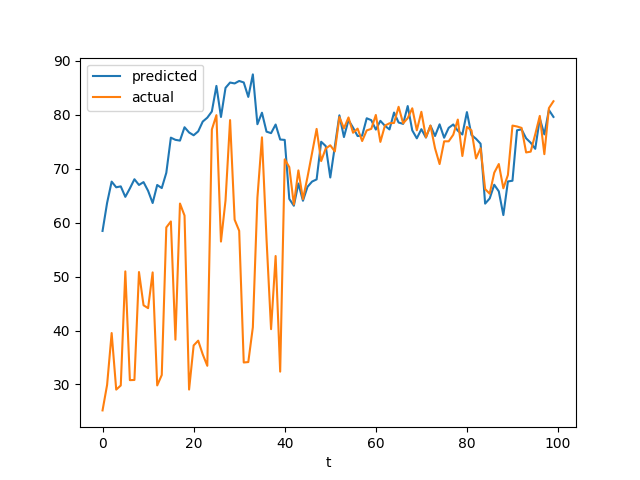
\includegraphics[width=\textwidth]{results/evaluation/f_model_graph_p80.png}
        \end{subfigure}
        \begin{subfigure}{\figwidth}
                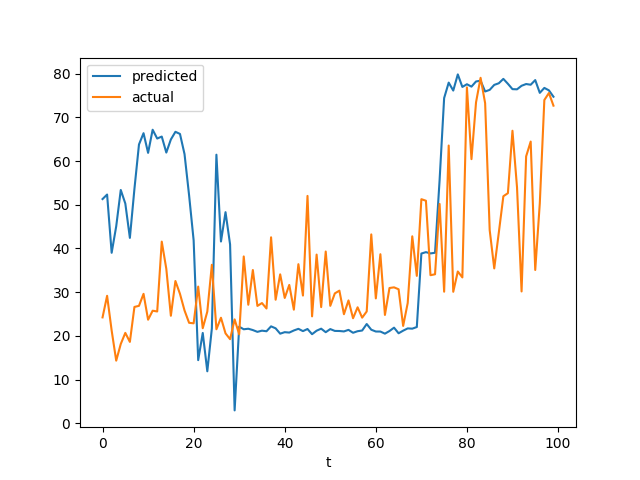
\includegraphics[width=\textwidth]{results/evaluation/f_model_graph_p90.png}
        \end{subfigure}
        \begin{subfigure}{\figwidth}
                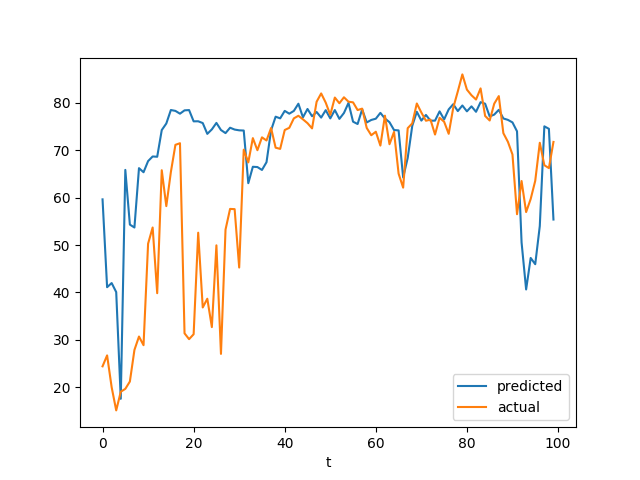
\includegraphics[width=\textwidth]{results/evaluation/f_model_graph_p100.png}
        \end{subfigure}
        \caption{Example time series predictions of the fuel models}
        \label{fig:fuel-prediction-examples}
    \end{figure}

    \begin{figure}
        \centering

        \begin{subfigure}{\figwidth}
            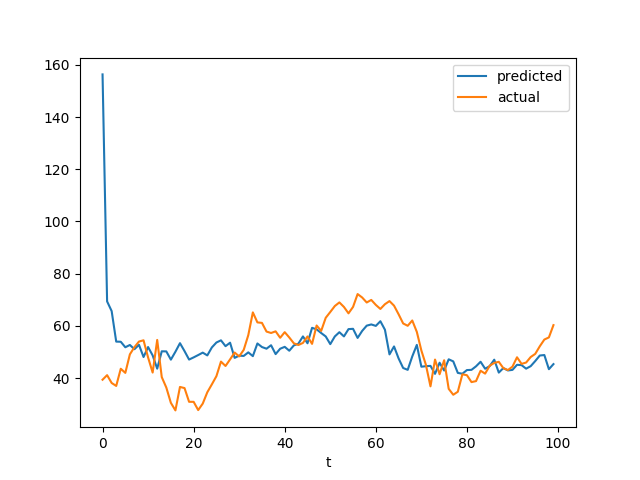
\includegraphics[width=\textwidth]{results/evaluation/c_model_graph_p10.png}
        \end{subfigure}
        \begin{subfigure}{\figwidth}
            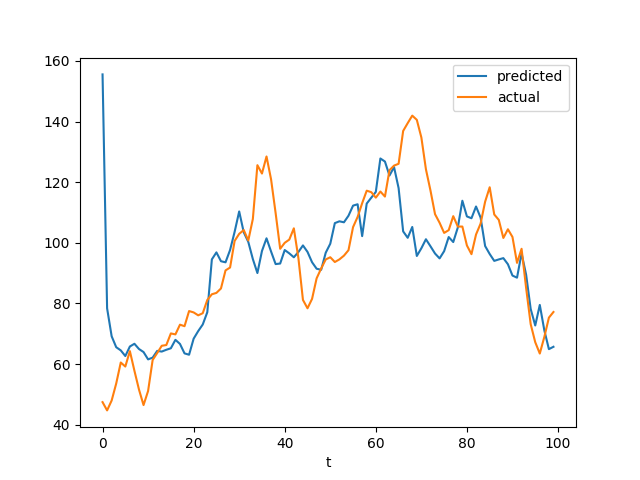
\includegraphics[width=\textwidth]{results/evaluation/c_model_graph_p20.png}
        \end{subfigure}
        \begin{subfigure}{\figwidth}
            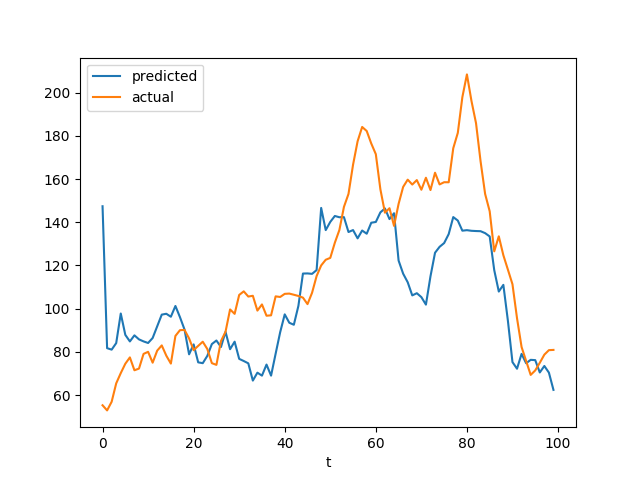
\includegraphics[width=\textwidth]{results/evaluation/c_model_graph_p30.png}
        \end{subfigure}
        \begin{subfigure}{\figwidth}
            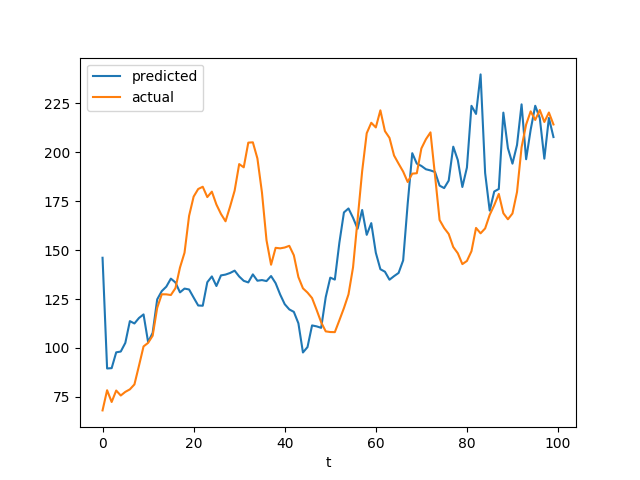
\includegraphics[width=\textwidth]{results/evaluation/c_model_graph_p40.png}
        \end{subfigure}
        \begin{subfigure}{\figwidth}
            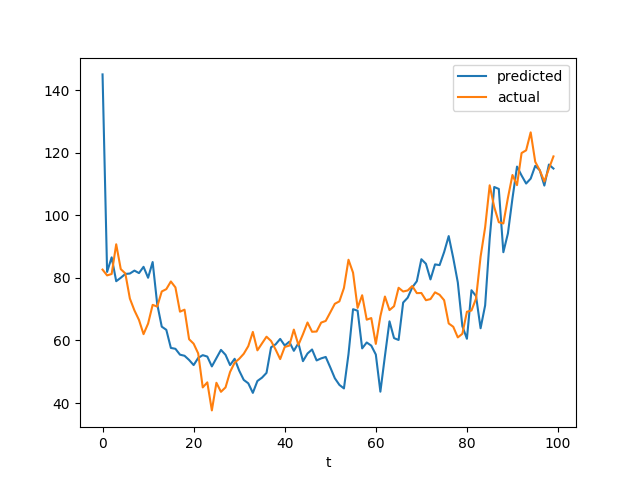
\includegraphics[width=\textwidth]{results/evaluation/c_model_graph_p50.png}
        \end{subfigure}
        \begin{subfigure}{\figwidth}
            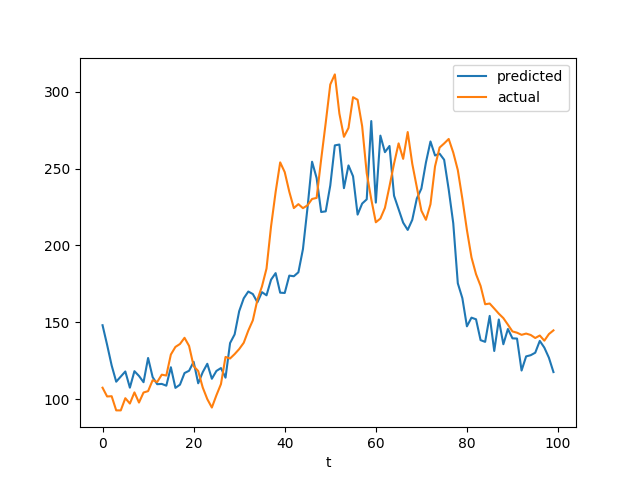
\includegraphics[width=\textwidth]{results/evaluation/c_model_graph_p60.png}
        \end{subfigure}
        \begin{subfigure}{\figwidth}
            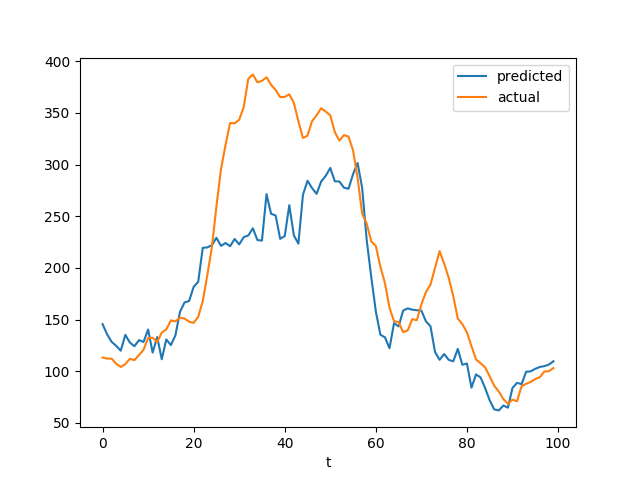
\includegraphics[width=\textwidth]{results/evaluation/c_model_graph_p70.png}
        \end{subfigure}
        \begin{subfigure}{\figwidth}
            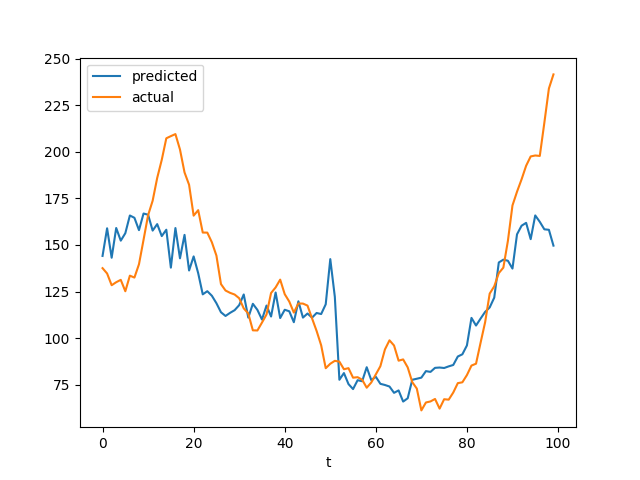
\includegraphics[width=\textwidth]{results/evaluation/c_model_graph_p80.png}
        \end{subfigure}
        \begin{subfigure}{\figwidth}
            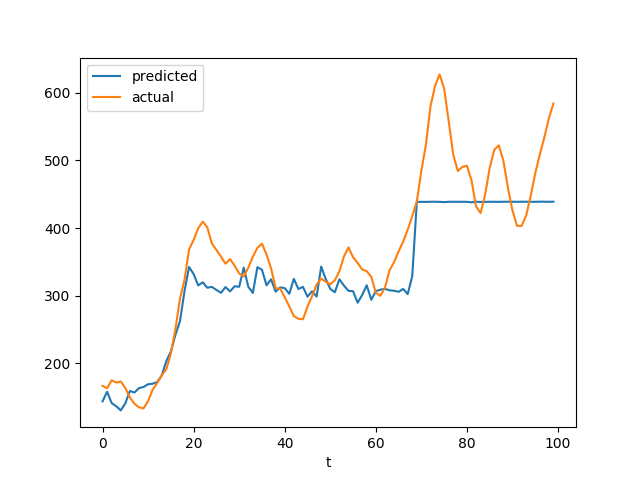
\includegraphics[width=\textwidth]{results/evaluation/c_model_graph_p90.png}
        \end{subfigure}
        \begin{subfigure}{\figwidth}
            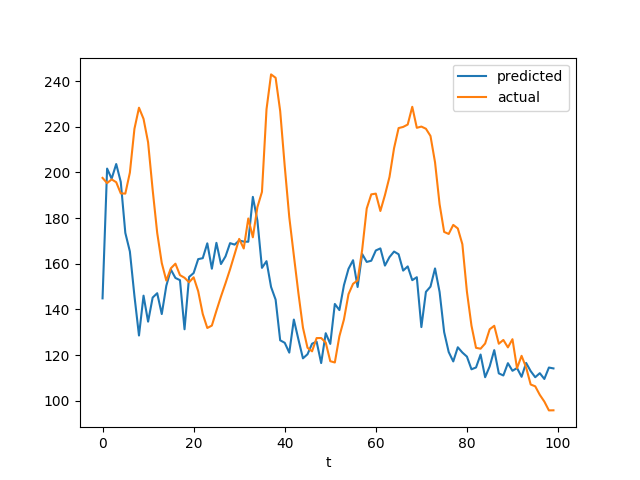
\includegraphics[width=\textwidth]{results/evaluation/c_model_graph_p100.png}
        \end{subfigure}
        \caption{Example time series predictions of the consumption models}
        \label{fig:consumption-prediction-examples}
    \end{figure}

\bibliographystyle{splncs04}
\bibliography{references.bib}

\end{document}
